\subsection{Định nghĩa cơ bản}


\begin{definition}[Đồ thị]
    Một đồ thị $G$ gồm một cặp thứ tự $(V(G),E(G))$, trong đó tập $V(G) \neq \varnothing $ là tập hợp các đỉnh và tập $E(G)$ được gọi là tập cạnh,
    mỗi cạnh nối 2 đỉnh là 2 thành phần của $V(G)$.
    $|V(G)|$ là số đỉnh trong tập kí hiệu bởi $\nu$ và $|E(G)|$ là số cạnh kí hiệu bởi $\epsilon$.
    Chú ý, tập $E(G)$ có thể rỗng, và một cạnh có thể nối 1 đỉnh đến chính nó.
\end{definition}

\begin{definition}[Khuyên]
    Khuyên là một cạnh bắt đầu và kết thúc tại cùng 1 đỉnh.
\end{definition}

\begin{definition}
    Đồ thị vô hướng $G(V(G),E(G))$ gọi là đơn đồ thị nếu $G$ không có khuyên và mỗi cặp đỉnh khác nhau $a,b \in V(G)$ được nối với nhau bởi không quá một cạnh.
\end{definition}
\begin{definition}
    Một đỉnh là liên thuộc với một cạnh nếu đỉnh đó là một trong 2 đầu mút của cạnh; hai đỉnh được gọi là kề nhau nếu chúng được nối bởi 1 cạnh.
    Bậc của một đỉnh $v$, kí hiệu bởi $deg(v)$, là số các cạnh liên thuộc với $v$, trong đó khuyên được tính như hai cạnh. Bậc của đồ thị là tổng bậc tất cả các đỉnh.
    Ta gọi $\delta = \displaystyle\min_{v \in V}(deg (v))$ và $\Delta = \displaystyle\max_{v \in V}(deg (v))$.
\end{definition}

\begin{definition}[Liên thông]
    Một đường đi $W$ trong $G$ là một dãy luân phiên các đỉnh và cạnh, biểu thị bởi $W=v_0e_1v_1e_2....e_kv_k$ trong đó $e_i (i \in [1,k], i \in \mathbb{N})$ nối giữa đỉnh $v_{i-1}$ và $v_i$.
    Một đường đi mà tất cả cách cạnh $e_i$ khác nhau gọi là đường đi đơn.
    Hơn nữa, nếu tất cả các đỉnh $v_i$ phân biệt thì $W$ là đường đi sơ cấp.
    Đồ thị $G$ liên thông nếu tồn tại một đường đi sơ cấp nối giữa mọi cặp đỉnh trong $G$.

    Một đường đi là đường đi đóng nếu nó có độ dài dương và điểm đầu trùng điểm cuối.

    Một đường đi đơn đóng với các đỉnh phân biệt được gọi là chu trình.
\end{definition}
\begin{remark}
    Trong phạm vi bài viết này, nếu chỉ nói đường đi mà không nói gì thêm tức là đường đi sơ cấp.
\end{remark}
\begin{definition}
    $H$ là đồ thị con của $G$ nếu $V(H) \subseteq V(G), E(H) \subseteq E(G)$ và đầu mút các cạnh trong $E(H)$ thuộc $V(H)$.
    Một thành phần liên thông của một đồ thị vô hướng là một đồ thị con trong đó giữa bất kì hai đỉnh nào đều có đường đi đến nhau, và nếu nhận thêm bất kỳ đỉnh nào sẽ mất tính liên thông.
    Số các thành phần liên thông của $G$ được biểu diễn bởi $\omega(G)$. Một cạnh $e$ được gọi là cầu nếu $\omega(G-e) > \omega(G)$
\end{definition}
\begin{center}
    \begin{tikzpicture}
        \foreach \x/\y in {0/0, 1.5/1, 3/0, 1.5/3} {
                \filldraw[black] (\x,\y) circle (2pt);
                \foreach \z/\t in {0/0, 1.5/1, 3/0, 1.5/3} {
                        \draw[black, thick] (\x,\y) -- (\z,\t);
                    }
            }
        \node at (1.5,-1,0) {Đồ thị ban đầu};
    \end{tikzpicture}
\end{center}

\begin{center}
    \begin{tikzpicture}
        \filldraw[black] (0,0) circle (2pt);
        \filldraw[black] (1.5,3) circle (2pt);
        \filldraw[black] (3,0) circle (2pt);
        \draw[black, thick] (0,0) -- (1.5,3);

        \filldraw[black] (7,0) circle (2pt);
        \filldraw[black] (8.5,3) circle (2pt);
        \filldraw[black] (10,0) circle (2pt);
        \draw[black, thick] (7,0) -- (8.5,3);
        \draw[black, thick] (10,0) -- (8.5,3);
        \draw[black, thick] (10,0) -- (7,0);

        \filldraw[black] (14,0) circle (2pt);
        \filldraw[black] (15.5,3) circle (2pt);
        \filldraw[black] (17,0) circle (2pt);
        \filldraw[black] (15.5,1) circle (2pt);
        \draw[black, thick] (14,0) -- (15.5,3);
        \draw[black, thick] (14,0) -- (15.5,1);
        \draw[black, thick] (15.5,3) -- (15.5,1);
        \draw[black, thick] (17,0) -- (15.5,3);
        \node at (8.5, -1, 0) {3 đồ thị con};
    \end{tikzpicture}
\end{center}

\begin{definition}
    Đồ thị đầy đủ là đồ thị đơn mà mỗi cặp đỉnh khác nhau được nối với nhau bởi duy nhất một cạnh. Kí hiệu $K_m$ là đồ thị đầy đủ $m$ đỉnh.

    Đồ thị G là đồ thị phân đôi nếu tập đỉnh $V$ của nó có thể chia thành hai tập con khác rỗng $X$ và $Y$ sao cho mọi cạnh trong $G$ nối một đỉnh trong $X$ với một đỉnh trong $Y$.

    Đồ thị G là đồ thị phân đôi đầy đủ nếu $\forall x \in X, y \in Y$ thì $x$ được nối với $y$ bởi một cạnh duy nhất.
    Khi $X$ chứa $m$ đỉnh, $Y$ chứa $n$ đỉnh thì $G$ kí hiệu bởi $K_{m,n}$.
    \begin{center}
        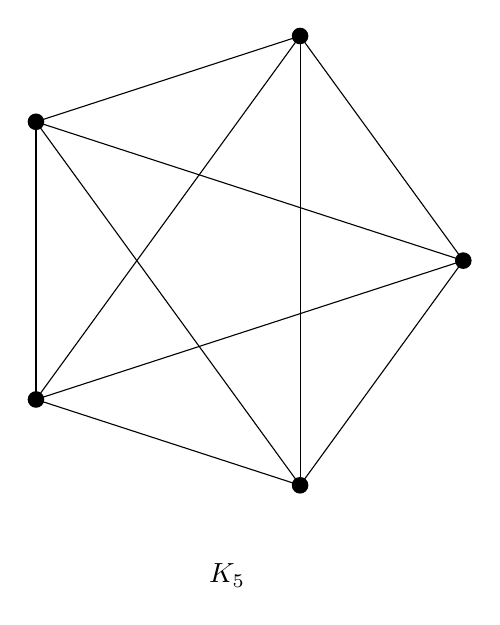
\begin{tikzpicture}
            \foreach \i in {1, 2, 3, 4, 5}
            \fill[black] (\i*360/5:3) coordinate (5\i) circle(3 pt)
            \ifnum \i>1 foreach \j in {\i,...,1}{(5\i) edge (5\j)} \fi;

            \node at (0,-4,0) {$K_5$};
        \end{tikzpicture}
        \hspace{2cm}
        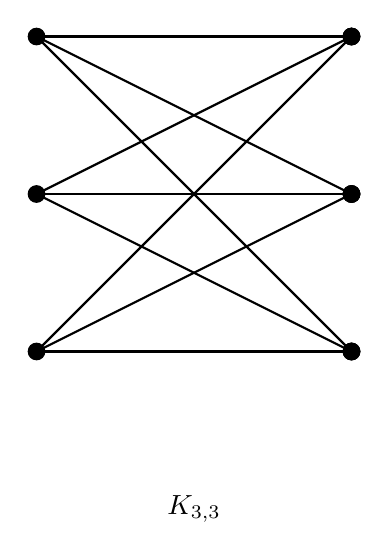
\begin{tikzpicture}
            \foreach \x/\y in {0/1, 0/3, 0/5} {
                    \filldraw[black] (\x,\y) circle (3pt);
                    \foreach \z/\t in {4/1, 4/3, 4/5} {
                            \filldraw[black] (\z,\t) circle (3pt);
                            \draw[black, thick] (\x,\y) -- (\z,\t);
                        }
                }
            \node at (2,-1,0) {$K_{3,3}$};
        \end{tikzpicture}
    \end{center}
\end{definition}
\begin{theorem}
    \label{thr:v2e}
    Cho đồ thị $G$ với tập đỉnh $V$ và tập cạnh $E$, $$\sum_{v\in V}deg(v) = 2\epsilon$$
\end{theorem}
\begin{proof}

    Giả sử $x,y \in V$ và $(x,y) \in E$

    \indent Với $x \neq y$, khi đó nếu xóa cạnh $(x,y)$ thì bậc của đồ thị giảm đi 2. Nếu ta xóa tất cả các cạnh như trên thì đồ thị còn lại chỉ gồm các đỉnh cô lập và các đỉnh có khuyên.

    Tại mỗi đỉnh $x$ có khuyên, nếu ta xóa khuyên, thì bậc của đồ thị cũng sẽ giảm đi 2

    Như vậy, sau khi xóa 1 cạnh nối 2 đỉnh khác nhau hoặc xóa 1 khuyên, thì bậc của đồ thị giảm đi 2. Sau khi xóa tất cả cách cạnh và các khuyên của đồ thị, thì đồ thị chỉ còn lại các đỉnh cô lập nên bậc đồ thị bằng 0.

    Từ đó, suy ra điều phải chứng minh
    %     Với $v\in V, e \in E$ gọi $n(v)$ là tập các cạnh liên thuộc với $v$. Gọi $m(e)$ là tập các đầu mút của $e$.
    %     Ta có: $$\sum_{v \in V}deg(v) = \sum_{v \in V}(\sum_{e \in n(v)}1) = \sum_{e \in E}(\sum_{v \in m(e)}1) = 2\epsilon$$
\end{proof}
\begin{definition}[Đồ thị phân chia]
    \label{def:subdivision}
    \textit{Chia nhỏ} cạnh $uv$ là phép toán thay thế cạnh $uv$ bằng 2 cạnh $uw$ và $wv$, đỉnh mới $w$ được thêm vào đồ thị ban đầu.
    Một đồ thị phân chia của đồ thị $G$ là đồ thị đạt được bằng cách \textit{chia nhỏ} cạnh trên $G$.
\end{definition}
\begin{figure}[H]
    \centering
    \begin{tikzpicture}
        \foreach \x/\y in {0/0, 1.5/1, 3/0, 1.5/3} {
                \filldraw[black] (\x,\y) circle (2pt);
                \foreach \z/\t in {0/0, 1.5/1, 3/0, 1.5/3} {
                        \draw[black, thick] (\x,\y) -- (\z,\t);
                    }
            }
        \node at (1.5,-1,0) {Đồ thị ban đầu};
        \node at (1.5,0.5,0) {$u$};
        \node at (1.5,3.5,0) {$v$};
    \end{tikzpicture}
    \hspace{2cm}
    \begin{tikzpicture}
        \foreach \x/\y in {0/0, 1.5/1, 3/0, 1.5/3} {
                \foreach \z/\t in {0/0, 1.5/1, 3/0, 1.5/3} {
                        \draw[black, thick] (\x,\y) -- (\z,\t);
                    }
            }
        \node at (1.5,-1,0) {Đồ thị phân chia};
        \node at (1.5,0.5,0) {$u$};
        \node at (1.5,3.5,0) {$v$};
        \node at (1.75,2,0) {$w$};
        \draw[blue, thick] (1.5,1) -- (1.5,3);
        \filldraw[purple] (1.5,2) circle (2pt);
        \foreach \x/\y in {0/0, 1.5/1, 3/0, 1.5/3} {
                \filldraw[black] (\x,\y) circle (2pt);
            }
    \end{tikzpicture}
\end{figure}

\begin{definition}
    \label{def:kcn}
    Cho đồ thị $G$, \textit{tập cắt} $V' \subseteq V$ là tập các đỉnh mà khi loại bỏ chúng sẽ làm cho đồ thị mất tính liên thông (khi \textit{loại bỏ} một đỉnh, ta loại bỏ cả những cạnh liên thuộc đỉnh đó).
    \textit{Bậc liên thông} của $G$, kí hiệu $\kappa(G)$, $\kappa(G) = |V'|$ với $V'$ là \textit{tập cắt} có ít phần tử nhất. Đồ thị $G$ là k-liên thông nếu $k \leq \kappa(G)$.
\end{definition}
\begin{center}
    \begin{tikzpicture}
        \draw[black, thick] (0,0) -- (0,4);
        \draw[black, thick] (0,0) -- (4,4);
        \draw[black, thick] (4,0) -- (4,4);
        \draw[black, thick] (2,2) -- (4,4);
        \draw[black, thick] (2,2) -- (2,4);
        \draw[black, thick] (0,4) -- (4,4);
        \draw[black, thick] (0,4) -- (4,0);
        \foreach \x/\y in {0/0, 0/4, 2/2, 2/4, 4/0, 4/4} {
                \filldraw[black] (\x,\y) circle (2pt);
            }
        \node at (2,-1,0) {Đồ thị 2-liên thông};
    \end{tikzpicture}
    \hspace{2cm}
    \begin{tikzpicture}
        \draw[black, thick] (0,0) -- (0,4);
        \draw[black, thick] (0,0) -- (4,4);
        \draw[black, thick] (4,0) -- (4,4);
        \draw[black, thick] (2,2) -- (4,4);
        \draw[black, thick] (0,4) -- (4,0);
        \draw[pink, thick] (2,2) circle (0.5);
        \foreach \x/\y in {0/0, 0/4, 2/2, 4/0, 4/4} {
                \filldraw[black] (\x,\y) circle (2pt);
            }
        \node at (2,-1,0) {Không phải 2-liên thông};
    \end{tikzpicture}
\end{center}